\providecommand{\main}{../main2}
\documentclass[\main/main.tex]{subfiles}
\setcounter{section}{4}
\graphicspath{{../images/}}
\begin{document}

\section{代数的Bethe仮設}
\begin{frame}{six-vertex model}
    まずsix-vertex modelを紹介する.これは2次元の氷をモデル化したものである.
    \begin{figure}[H]
        \centering
        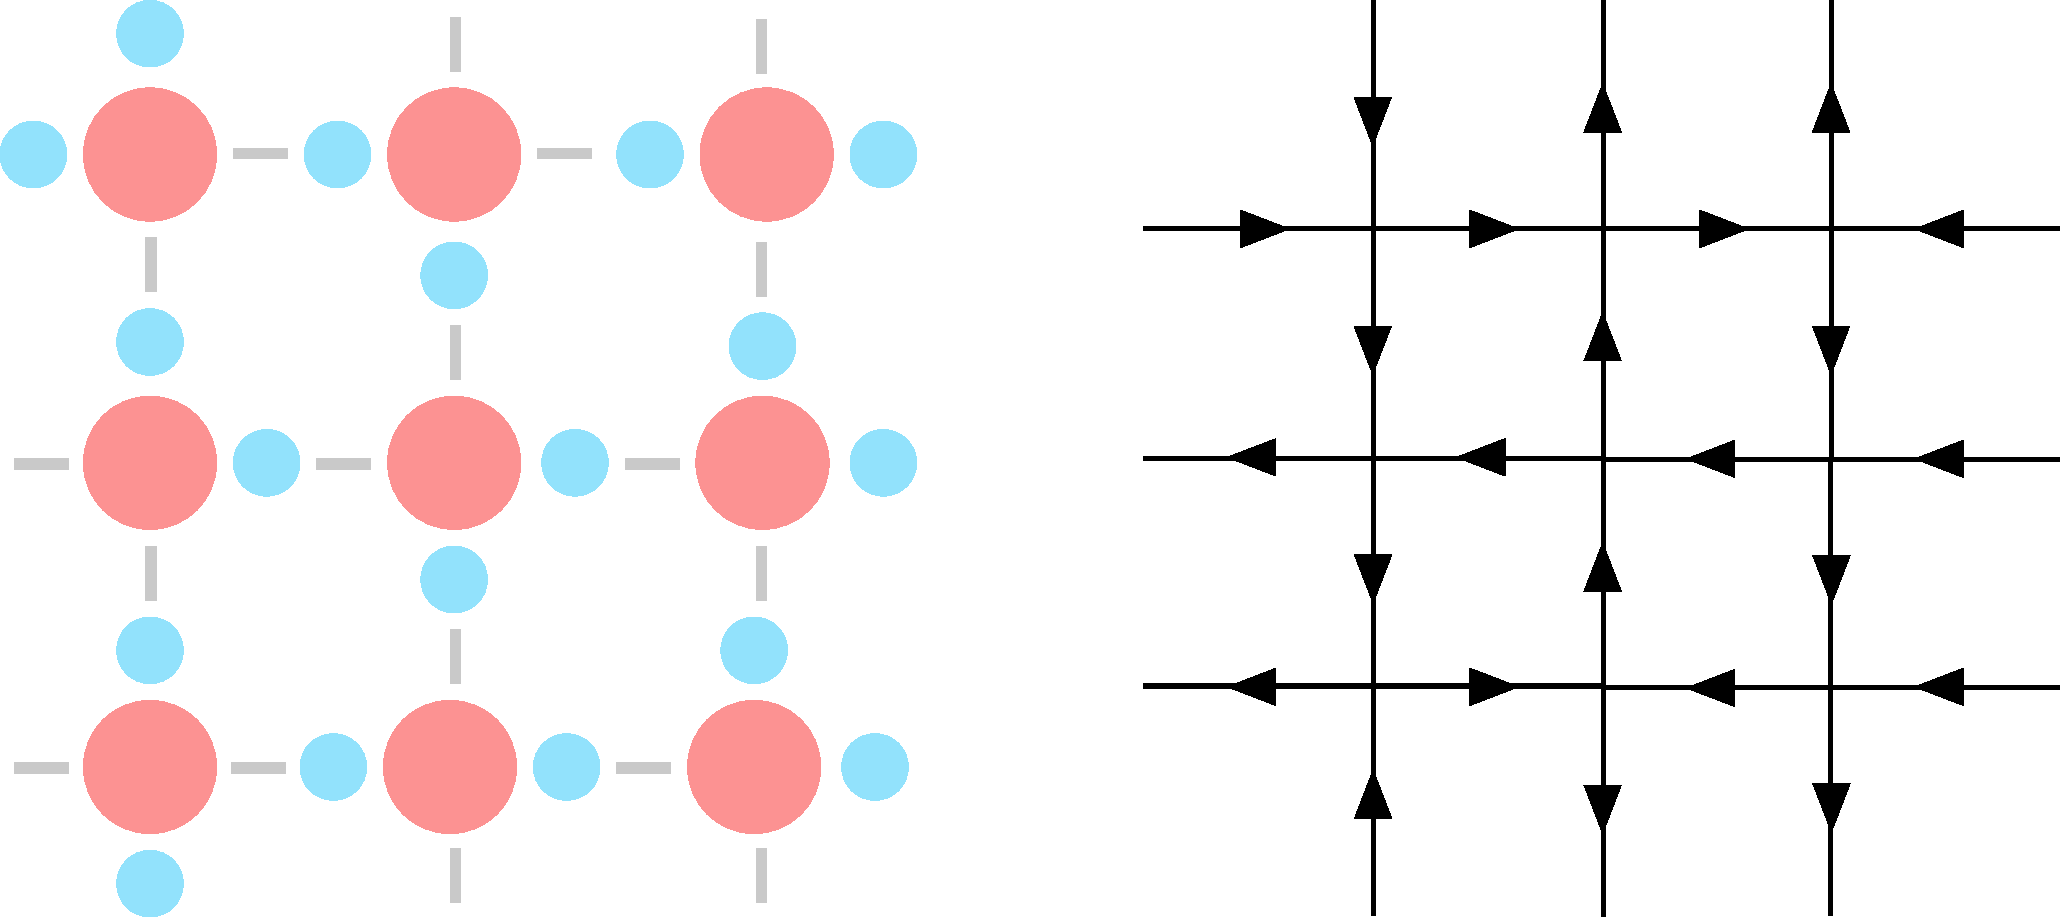
\includegraphics[scale = 0.2]{2DIce.pdf}
    \end{figure}
    左の図では,正方格子の各辺で水素原子の配置に2通りの自由度が存在する.これを頂点を結ぶ矢印として書いたのが右の図である.

    各頂点が電気的に中性であるという条件を課すと,各頂点で流入する矢印と流出する矢印の数が等しくなる.これをice ruleという.
\end{frame}

\begin{frame}
    Ice rule を考慮すると,あり得る頂点は6通り存在する.ここからこの模型をsix-vertex modelと呼ぶ.
    矢印の反転に対する対称性を仮定すると,Boltzmann weight $a,b,c$によって模型は決定される.
    \begin{figure}[H]
        \centering
        \includegraphics[scale = 0.25]{6vertex.pdf}
    \end{figure}
    ここで,右向き・上向きの矢印を正とし,左向き・下向きの矢印を負とした.
    % Boltzmann weightは普通$e^{-\beta E}$という形で書かれるが,ここでは温度依存性に注目しないのでまとめて記号$a, b, c$でおいた.
    Boltzmann weight全体を定数倍しても,分配関数は変わらないので,$a, b, c$は自由に規格化してよい.
    % 分配関数の計算は,あらゆる矢印の配位について,各頂点でのBoltzmann weightの積を足し合わせることで行われる.
\end{frame}

\begin{frame}
    six-vertex modelの頂点は,上下左右の矢印の符号に対して,$0,a,b,c$のいずれかを返すようなテンソルだとみなせる.
    $\alpha$行目,$n$列目の頂点を,2つのスピンの合成系に対する演算子として,L演算子を
    \begin{align}
        L_{\alpha,n} &
        = \frac{a+b}{2} 1_\alpha 1_n + \frac{a-b}{2} \sigma_\alpha^z \sigma_n^z + \frac{c}{2}(\sigma_\alpha^- \sigma_n^+ + \sigma_\alpha^+ \sigma_n^-)
        \\[5pt] &
        = \frac{1}{2}\mqty(
            a(1+\sigma_n^z) + b(1-\sigma_n^z) & 
            c\sigma_n^- \\
            c\sigma_n^+ &
            a(1-\sigma_n^z) + b(1+\sigma_n^z)
            )
        \\[5pt] &
        = \mqty(
            a&0&0&0 \\
            0&b&c&0 \\
            0&c&b&0 \\
            0&0&0&a
        )
    \end{align}
    と定義する.
    ここで,$\bra{k}_\alpha \bra{j}_n   L_{\alpha,n} \ket{i}_n \ket{l}_\alpha = (  L_{\alpha,n})^i_j|_{kl}$は頂点$(\alpha,n)$のBoltzmann weightであり,添字$i,j,k,l$はそれぞれ上下左右の矢印の符号を表している.
\end{frame}

\begin{frame}{}
      モノドロミー行列$T$および転送行列$\tau$は,$\alpha$行目の頂点$(\alpha,1),\ldots,(\alpha,N)$に対し,
    \begin{gather}
        (T_\alpha)_{kl} = (L_{\alpha,1} L_{\alpha,2} \cdots L_{\alpha,N})_{kl} 
        \\[5pt]
        \tau_\alpha = \tr T_\alpha = \sum_{i} (L_{\alpha,1} L_{\alpha,2} \cdots L_{\alpha,N})_{kk}
    \end{gather}
    と定義される.$\alpha$についての添字は支障がなければ省略する.
    モノドロミー行列は$T_{j_1j_2\cdots j_N}^{i_1i_2\cdots i_N}|_{kl}$という添字をもち,転送行列は$\tau_{j_1j_2\cdots j_N}^{i_1i_2\cdots i_N}$という添字をもつ.
    上下方向に並んだ転送行列$\tau$を全て掛け合わせてトレースをとれば分配関数が得られる:
    \begin{align}
        Z = \tr(\tau^N) = \sum_{i_1,\ldots,i_N} (\tau^N)_{i_1 \cdots i_N}^{i_1 \cdots i_N}.
    \end{align}
    したがって分配関数を求めるためには,$\tau$の固有値が分かればよい.
\end{frame}

\begin{frame}{XXZ modelとの対応}
    $a,b,c$を以下のようなパラメーター$\lambda,\eta \in \mathbb{C}$で表すと便利である.
    \begin{align}
        \begin{cases}
            a = \sin (\lambda + 2\eta)
            \\
            b = \sin (\lambda)
            \\
            c = \sin (2\eta)
        \end{cases},
        \quad
        \begin{cases}
            a = \lambda + 2\eta
            \\
            b = \lambda
            \\
            c = 2\eta
        \end{cases},
        \quad
        \begin{cases}
            a = \sinh (\lambda + 2\eta)
            \\
            b = \sinh (\lambda)
            \\
            c = \sinh (2\eta)
        \end{cases}
    \end{align}
    パラメーター表示の使い分けは,
    \begin{align}
        \Delta = \frac{a^2+b^2-c^2}{2ab} = \cos(2\eta),~ 1,~ \cosh(2\eta)
    \end{align}
    によって行う.$|\Delta| < 1$の場合は左,$\Delta = 1$の場合は真ん中,$\Delta > 1$の場合は右を採用する.$\Delta \le -1$の場合は今は考えない.
    具体的な計算は$|\Delta| < 1$の場合で行うが,その他の場合も結果は同じである.
\end{frame}

\begin{frame}{}
    L演算子$L_{\alpha,n}$を
    \begin{align}
          L_{\alpha,n} = \mqty(
            1&0&0&0 \\
            0&b/a&c/a&0 \\
            0&c/a&b/a&0 \\
            0&0&0&1
        )
    \end{align}
    と定義し直す.
    実は,$XXZ$ modelのハミルトニアンとsix-vertex modelの転送行列の間には,
    \begin{align}
        H_{XXZ} = \frac{\sin(2\eta)}{2}\dv{\lambda} \ln \tau(\lambda) \eval_{\lambda = 0} + \frac{1}{4}N\cos(2\eta)
    \end{align}
    という関係が成り立つ.これを証明しよう.
    \begin{align}
        \dv{\lambda}\ln\tau(\lambda) = \tau(\lambda)^{-1} \dv{\lambda}\tau(\lambda)
    \end{align}
    より,$\tau^{-1}(0)$と$\tau'(0)$をそれぞれ求めることにする.
\end{frame}

\begin{frame}{}
    $\lambda = 0$のとき,$b = 0,~ a = c = \sin(2\eta)$となる.したがって,
    \begin{align}
          L_{\alpha,n}(\lambda = 0)
        = \mqty(
            1&0&0&0\\
            0&0&1&0\\
            0&1&0&0\\
            0&0&0&1
        )
        = \Pi^{(\alpha,n)}
    \end{align}
    と書ける.$L_n(0)$を掛け合わせてトレースをとることで,転送行列$\tau(0)$が求まる.これは以下のように図示すると分かりやすい.
    \begin{align}
        \tau = ~
        \Includegraphics[scale = 0.4, trim = 0 0 0 0.3cm]{tau.pdf}
    \end{align}
    すなわち,$\tau(0)$は全ての格子のスピンを左にシフトさせるような演算子である.
    よって$\tau^{-1}(0)$は,スピンを右にシフトさせることがわかる.
\end{frame}

\begin{frame}
    つぎに$\tau'(0)$を求める.$\lambda=0$のとき,
    % $a'=\cos(2\eta),~b'=1,~c'=0$となる.したがって,
    \begin{align}
        \dv{\lambda}\qty\Big(\frac{b}{a})\eval_{\lambda=0} = \frac{1}{\sin(2\eta)},
        \quad
        \dv{\lambda}\qty\Big(\frac{c}{a})\eval_{\lambda=0} = -\frac{\cos(2\eta)}{\sin(2\eta)}
    \end{align}
    となることから,
    \begin{align}
          L_{\alpha,n}'(\lambda = 0) &= \frac{1}{\sqrt{|1-\Delta^2|}}\mqty(
            0&0&0&0\\
            0&1&-\Delta&0\\
            0&-\Delta&1&0\\
            0&0&0&0
        )
        % \\ &
        % = \frac{1}{2\sin(2\eta)}(1_01_n - \sigma_0\sigma_z - \Delta\sigma_0^+\sigma_n^+ - \Delta\sigma_0^+\sigma_0^-)
    \end{align}
    と書ける.
\end{frame}

\begin{frame}{}
    以上の結果から,
    \begin{figure}[H]
        \centering
        \includegraphics[scale = 0.35]{Baxter_formula.pdf}
    \end{figure}
    となる.$\Sigma$の中身を計算すると,
    \begin{align}
        \Pi^{(n,n+1)}  L_{n+1,n}'(0)
        = \frac{1}{\sqrt{|1-\Delta^2|}}\mqty(
            0&0&0&0\\
            0&-\Delta&1&0\\
            0&1&-\Delta&0\\
            0&0&0&0
        ).
        \label{XXZ model: interaction}
    \end{align}
\end{frame}

\begin{frame}{}
    (\ref{XXZ model: interaction})を$n$について足し合わせると,
    \begin{align}
        &\nonumber
        \dv{\lambda}\ln\tau(\lambda)\eval_{\lambda=0}
        \\ &
        = \frac{1}{\sqrt{|1-\Delta^2|}} \sum_{n=1}^N \qty[
            \Delta \frac{\sigma_n^z \sigma_{n+1}^z - 1_n 1_{n+1}}{2} + \frac{\sigma_n^+\sigma_n^- + \sigma_n^- \sigma_n^+}{4}
        ].
    \end{align}
    したがって,
    \begin{align}
        H_{XXZ} 
        % = \sum_{n=1}^N (S_n^x S_{n+1}^x + S_n^y S_{n+1}^y + \Delta S_n^z S_{n+1}^z)
        = \frac{\sqrt{|1-\Delta^2|}}{2}\dv{\lambda}\ln\tau(\lambda)\eval_{\lambda=0} + \frac{1}{4}N\Delta
    \end{align}
    となって,目的の式が示された.この式は$\Delta>1$の場合にも成り立つ.
    $\Delta = 1$の場合は$\eta \to 0$の極限をとって,
    \begin{align}
        H_{XXX} = \eta \dv{\lambda}\ln\tau(\lambda)\eval_{\lambda=0} + \frac{1}{4}N.
    \end{align}
    となる.
\end{frame}

\begin{frame}{Yang-Baxter関係式}
    異なるBoltzmann weightから構成されるL演算子$L(\lambda), L(\mu)$に対し,以下の図で表されるような関係式を考えてみる.
    \begin{align}
        \Includegraphics[scale = 0.25]{YBE.pdf}
        \label{YBE}
    \end{align}
    ここで矢印は正の向きとする方向を表している.式で書くと,
    \begin{align}
        R(\lambda-\mu)(L_n(\lambda) \otimes L_n(\mu)) = (L_n(\mu)\otimes L_n(\lambda))R(\lambda-\mu)
    \end{align}
    である.$R(\lambda-\mu)$はR演算子と呼ばれ,ここではL演算子と同じである.
\end{frame}
\begin{frame}{}
    まずYang-Baxter関係式が成り立つと,何が嬉しいかを説明する.
    $R(\lambda-\mu)(T(\lambda) \otimes T(\mu))$を考え,Yang-Baxter関係式を繰り返し用いると,
    \begin{align*}
        \Includegraphics[scale = 0.15]{YBE-1.pdf}
        \quad &= \quad \Includegraphics[scale = 0.15]{YBE-2.pdf}
        \\[10pt] &
        =\quad \Includegraphics[scale = 0.15]{YBE-3.pdf} 
    \end{align*}
    両辺に$R^{-1}(\lambda-\mu)$を掛けてトレースをとることで,転送行列の間の交換関係
    \begin{align}
        [\tau(\lambda),\tau(\mu)] = 0
    \end{align}
    が得られる.
\end{frame}

\begin{frame}
    Yang-Baxter関係式を具体的に解いて,頂点
    が満たすべき条件を求めよう.
    まず,(\ref{YBE})を以下のように改変しておく.
    \begin{align}
        \Includegraphics[scale = 0.15]{YBE_rotate.pdf}
    \end{align}
    この変形は矢印の反転に対する対称性から従う.
    さらに,基準となる方向を反転して,
    \begin{align}
        \Includegraphics[scale = 0.15]{YBE_modified.pdf}
    \end{align}
    とする.これは2つの頂点(無印と白丸)で$a \leftrightarrow b$という変換をしたことを意味している.後で元に戻せば正しい結果を与える.
\end{frame}
\begin{frame}
    (\ref{YBE})は$2^6 = 64$個の方程式の集まりであるが,実際は3つの方程式で表せる.
    \begin{itemize}
        \item ice ruleのために,流入する矢印の数と流出する矢印の数は等しくなる.したがって,両辺が$0$でないのは${}_6 C_3 = 20$通りだけである.
        \item さらに矢印の反転に対する対称性から,$10$通りだけ考えれば良い.
        \item     $10$通りのうちの$4$通りでは,(\ref{YBE})の左辺と右辺がちょうど矢印を反転したものになり,恒等式を与える.これは,
        \begin{align}
            \mqty(j_1 & j_2 & j_3 \\ i_1 & i_2 & i_3) &\nonumber
            = \mqty(\mathrm{in} & \mathrm{in} & \mathrm{in} \\ \mathrm{out} &\mathrm{out} & \mathrm{out}),
            \quad
            \mqty(\mathrm{in} & \mathrm{out} & \mathrm{in} \\ \mathrm{out} &\mathrm{in} & \mathrm{out}),
            \\ &\qquad
            \mqty(\mathrm{out} & \mathrm{in} & \mathrm{in} \\ \mathrm{out} &\mathrm{out} & \mathrm{in}),
            \quad
            \mqty(\mathrm{in} & \mathrm{in} & \mathrm{out} \\ \mathrm{in} &\mathrm{out} & \mathrm{out})
        \end{align}
        という場合である.ただし,$\mathrm{in}$は流入する矢印を表し,$\mathrm{out}$は流出する矢印を表す.
        \item 残りの$6$通りから,$6$個の方程式が得られるが,左辺と右辺を入れ替えたものが出てくるので実質的な方程式の数は$3$個である.
    \end{itemize}
\end{frame}
\begin{frame}
    そのうちの1つは,
    \begin{figure}[H]
        \centering
        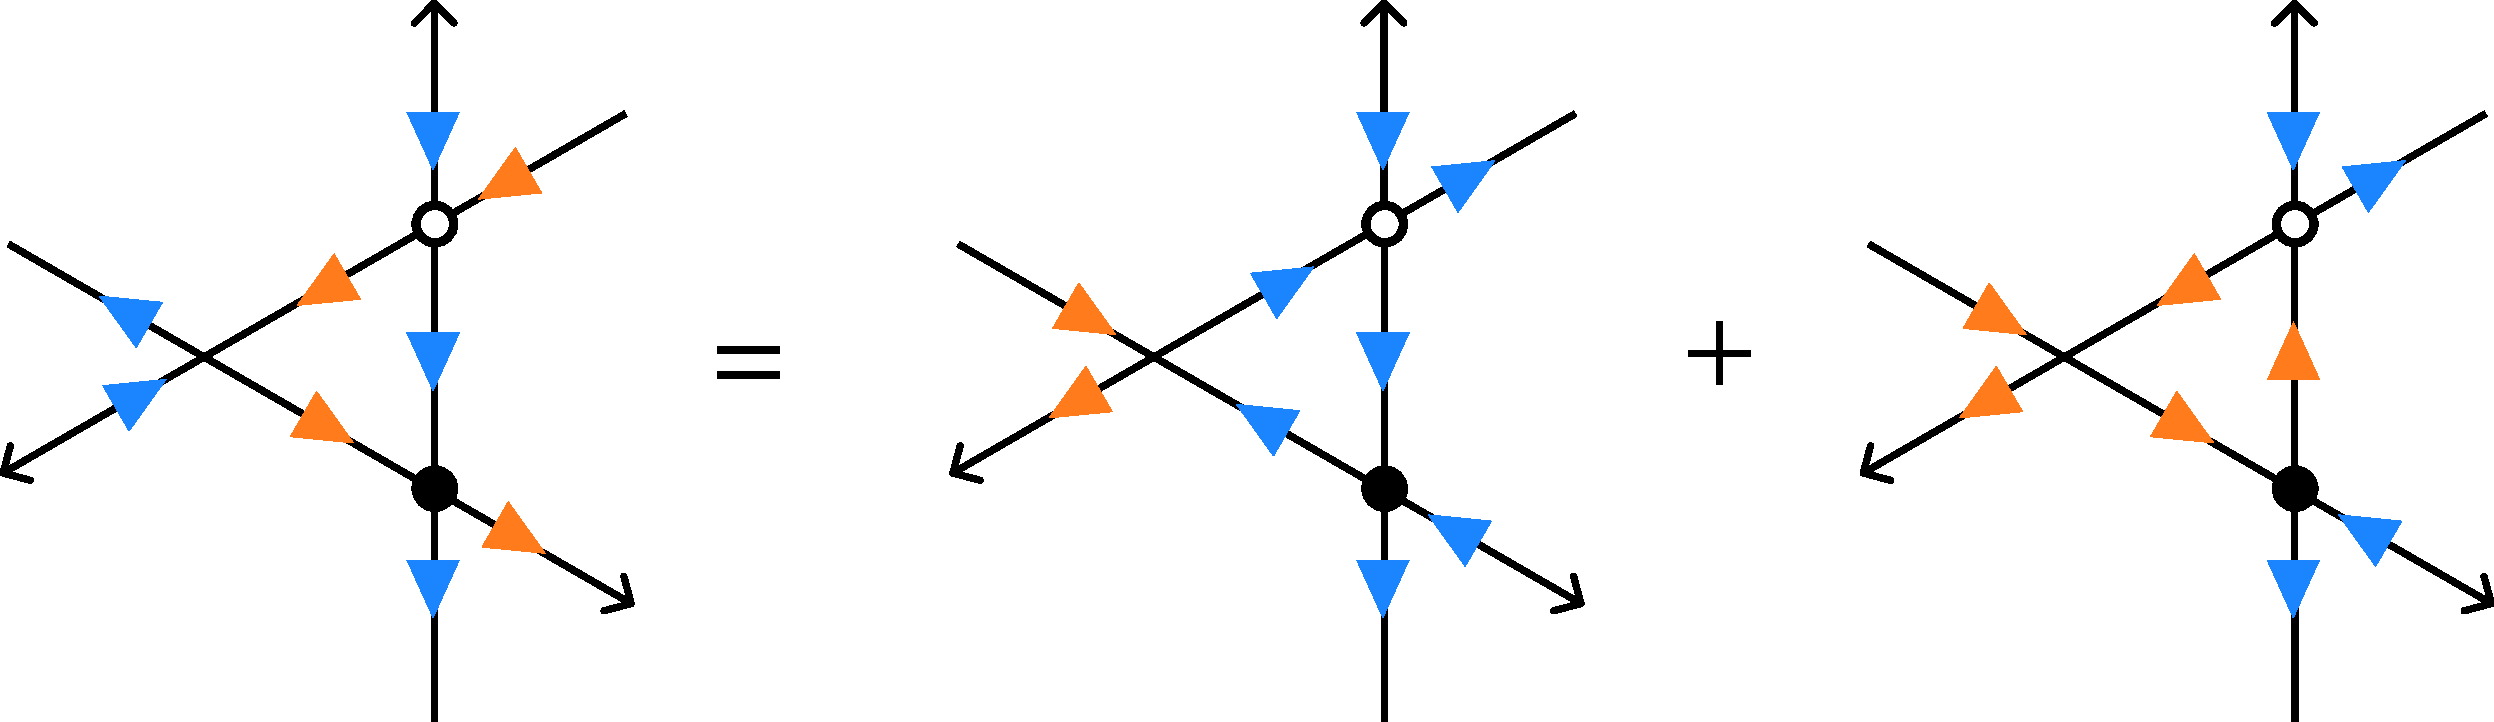
\includegraphics[scale = 0.2]{YBE_abc.pdf}
    \end{figure}
    という式で表される.$a(\lambda-\mu) = a,~ a(\lambda) = a',~ a(\mu) = a''$のようにおいて,Boltzmann weightを使って書くと,
    \begin{align}
        cb'b'' = ca'a'' + ac'c''
    \end{align}
    となる.頂点を巡回させることで,残りの方程式は以下のように求まる.
    \begin{align}
        bc'b'' = ac'a'' + ca'c''\\
        bb'c'' = aa'c'' + cc'a''
    \end{align}
\end{frame}

\begin{frame}{}
    自明でない解が存在する条件は,
    \begin{align*}
        &
        \det \mqty(
            ca' & -cb' & ac' \\
            ac' & -bc' & ca' \\
            cc' & 0    & aa'-bb'
        )
        \\ &
        = cc'(aa'-bb')(-a'b+ab') + cc'(-a'b'c^2+abc'^2)
        = 0.
    \end{align*}
    両辺を$2aa'bb'cc'$で割ると,
    \begin{align}
        \frac{a^2+b^2-c^2}{2ab} - \frac{a'^2+b'^2-c'^2}{2a'b'} \equiv \Delta - \Delta' = 0.
    \end{align}
    よって$\Delta = \Delta' = \Delta''$が分かる.またこの式は$a \leftrightarrow  b,~ a' \leftrightarrow b'$としても不変だから,もとのYang-Baxter関係式の解も同様である.
\end{frame}

\begin{frame}{代数的Bethe仮設}
    $\Delta = 1$の場合を考える.パラメーターのとり方を変えて,L演算子を
    \begin{align}
        L_n(\lambda) = 
        \mqty(
            \lambda + \eta\sigma_n^z & \eta\sigma_n^- \\
            \eta\sigma_n^+ & \lambda - \eta\sigma_n^z
        )
    \end{align}
    で定義する.これは今までの定義で$\lambda + \eta \to \lambda$としたものである.

    またモノドロミー行列の成分表示を
    \begin{align}
        T(\lambda) = L_1(\lambda) \cdots L_N(\lambda) = \mqty(A(\lambda)&B(\lambda)\\C(\lambda)&D(\lambda)) 
    \end{align}
    と書く.
\end{frame}

\begin{frame}{}
    モノドロミー行列の間の関係式
    \begin{align}
        R(\lambda - \mu) \cdot T(\lambda)\otimes T(\mu)
        = T(\mu) \otimes T(\lambda) \cdot R(\lambda-\mu)
    \end{align}
    から,16個の交換関係
    \begin{align}
        &\nonumber
         \mqty(
            a&0&0&0\\
            0&b&c&0\\
            0&c&b&0\\
            0&0&0&a
        ) \mqty
        (
            AA'&AB'&BA'&BB'\\
            AC'&AD'&BC'&BD'\\
            CA'&CB'&DA'&DB'\\
            CC'&CD'&DC'&DD'
        )
        \\ &
        = \mqty
        (
            A'A&A'B&B'A&B'B\\
            A'C&A'D&B'C&B'D\\
            C'A&C'B&D'A&D'B\\
            C'C&C'D&D'C&D'D
        ) \mqty(
            a&0&0&0\\
            0&b&c&0\\
            0&c&b&0\\
            0&0&0&a
        )
    \end{align}
    を得る.ただし,引数を省略して,$a = a(\lambda-\mu), A = A(\lambda), A' = A(\mu)$などと表した.
\end{frame}

\begin{frame}{}
    このうち使う交換関係は3つだけで,1行目4列目,1行目2列目,2行目4列目に注目すると,
    \begin{align}
        &
        B(\lambda) B(\mu) = B(\mu) B(\lambda)
        \\ &
        a(\lambda-\mu) A(\lambda)B(\mu) = b(\lambda-\mu) A(\mu)B(\lambda) + c(\lambda-\mu) B(\mu)A(\lambda)
        \\ &
        b(\lambda-\mu) B(\lambda)D(\mu) + c(\lambda-\mu) D(\lambda) B(\mu) = a(\lambda-\mu)B(\mu)D(\lambda)
    \end{align}
    を得る.
\end{frame}

\begin{frame}{}
    代数的Bethe仮設法においては,転送行列$\tau(\lambda)$の固有状態として,
    \begin{align}
        \ket{M} = B(\lambda_1)\cdots B(\lambda_M)\ket{0}
    \end{align}
    と書けるものを仮定する.
    まず真空$\ket{0} = \ket{\uparrow}_1 \ket{\uparrow}_2 \cdots \ket{\uparrow}_N$が$\tau(\lambda)$の固有状態であることを示す.
    \begin{align}
        L_n(\lambda)\ket{\uparrow}_n
        = \mqty(
            (\lambda+\eta)\ket{\uparrow}_n& \eta\ket{\downarrow}_n\\
            0&(\lambda-\eta)\ket{\uparrow}_n
            )
    \end{align}
    が上三角行列であることに注目すると,
    \begin{align}
        T(\lambda)\ket{0} = \mqty(A(\lambda)&B(\lambda)\\C(\lambda)&D(\lambda))\ket{0}
        = \mqty((\lambda+\eta)^N\ket{0}& * \\ 0 & (\lambda-\eta)^N\ket{0})
    \end{align}
    と書ける.トレースをとると,
    \begin{align}
        \tau(\lambda)\ket{0} = (\alpha(\lambda) + \delta(\lambda))\ket{0}.
    \end{align}
    ただし,$\alpha(\lambda) = (\lambda+\eta)^N,~ \delta(\lambda) = (\lambda-\eta)^N$と定義した.
\end{frame}

\begin{frame}{}
    次に,1粒子状態として,$B(\lambda_1)\ket{0}$を考える.
    \begin{align}
        \tau(\lambda)B(\lambda_1)\ket{0}
        = \qty[A(\lambda) + D(\lambda)]B(\lambda_1)\ket{0}
        \overset{?}{\propto} B(\lambda_1)\ket{0}
    \end{align}
    ここで,
    \begin{align}
        A(\lambda)B(\lambda_1)\ket{0}
        = \frac{a(\lambda_1-\lambda)}{c(\lambda_1-\lambda)}B(\lambda_1)\alpha(\lambda)\ket{0} + \frac{b(\lambda_1-\lambda)}{c(\lambda_1-\lambda)}B(\lambda)\alpha(\lambda_1)\ket{0}
    \end{align}
    である.同様に,
    \begin{align}
        D(\lambda)B(\lambda_1)\ket{0}
        = \frac{a(\lambda-\lambda_1)}{c(\lambda-\lambda_1)}B(\lambda_1)\delta(\lambda)\ket{0} + \frac{b(\lambda-\lambda_1)}{c(\lambda-\lambda_1)}B(\lambda)\delta(\lambda_1)\ket{0}
    \end{align}
    である.したがって,$B(\lambda_1)\ket{0}$が$\tau(\lambda)$の固有状態になるための条件として,
    \begin{align}
        \frac{b(\lambda_1-\lambda)}{c(\lambda_1-\lambda)}\alpha(\lambda_1) + \frac{b(\lambda-\lambda_1)}{c(\lambda-\lambda_1)}\delta(\lambda_1) = 0
        \label{ABA: 1particle BE}
    \end{align}
    が導かれる.
\end{frame}

\begin{frame}{}
    $b(\lambda)$は奇関数,$c(\lambda)$は偶関数なので,(\ref{ABA: 1particle BE})は
    \begin{align}
        \frac{\alpha(\lambda_1)}{\delta(\lambda_1)} = \qty(\frac{\lambda_1 + \eta}{\lambda_1 - \eta})^{N} = 1
    \end{align}
    となる.$\lambda_1$をリスケールすれば,
    \begin{align}
        \qty(\frac{\lambda_1 + i}{\lambda_1 - i})^N = 1
    \end{align}
    となる.これは1粒子状態に対するBethe仮設方程式である.
    さらに,2粒子状態が転送行列の固有状態となる条件
    \begin{align}
        \tau(\lambda)B(\lambda_1)B(\lambda_2)\ket{0} \propto B(\lambda_1)B(\lambda_2)\ket{0}
    \end{align}
    を考える.同様に交換関係を用いると,$\lambda_1, \lambda_2$に対する2粒子状態のBethe仮設方程式を得ることができる.
\end{frame}
\end{document}